\chapter{Đọc thêm 2: Trích xuất thông tin từ GDELT để phân tích thị trường trái phiếu chính phủ EU (Consoli và cộng sự)}
\label{ch:M5L3DocThem2}

\section{Thông tin nguồn}

\begin{itemize}
  \item \textbf{Nguồn:} Consoli, S., Tiozzo Pezzoli, L. \& Tosetti, E. ``Extracting Information from GDELT for EU Sovereign Bond Market Analysis.'' Springer, 2021.
  \item \textbf{Phần cần đọc:} tr. 55--67
  \item \textbf{Ghi chú:} bản chuyển ngữ tiếng Việt súc tích, bám cấu trúc nguồn (giữ nguyên tiêu đề, công thức, số liệu, bảng, chú thích và danh mục tài liệu tham khảo).
\end{itemize}

Sergio Consoli, Luca Tiozzo Pezzoli và Elisa Tosetti

Joint Research Centre, Directorate A - Strategy, Work Programme and Resources, Scientific Development Unit, European Commission, Via E. Fermi 2749, 21027 Ispra, VA, Italy; Department of Management, Università Ca\textquotesingle{} Foscari Venezia, Venice, Italy.

\textbf{Tóm tắt.} Bài viết giới thiệu tổng quan một dự án đang triển khai nhằm xây dựng phương pháp tạo các chỉ báo kinh tế - tài chính phản ánh cảm xúc của nhà đầu tư và mức độ phổ biến của các chủ đề, hữu ích cho việc phân tích thị trường trái phiếu chính phủ của các nước EU. Các chỉ báo thay thế này được lấy từ cơ sở dữ liệu Global Data on Events, Location, and Tone (GDELT), một kho dữ liệu mở, thời gian thực, quy mô lớn về xã hội loài người phục vụ nghiên cứu mở, theo dõi tin tức truyền hình, báo in và web trên toàn thế giới, tạo nên một nền tảng mở miễn phí để tính toán trên toàn bộ truyền thông thế giới. Sau phần tổng quan về phương pháp đang phát triển, bài trình bày một số kết quả sơ bộ cho trường hợp Ý. Kết quả cho thấy phương pháp ban đầu đạt hiệu quả tốt trong dự báo thị trường trái phiếu chính phủ Ý, sử dụng thông tin trích từ GDELT cùng mạng bộ nhớ dài-ngắn hạn sâu (Long Short-Term Memory) được huấn luyện và kiểm định theo cách tiếp cận cửa sổ trượt để phản ánh tốt nhất tính phi tuyến của dữ liệu.

\textbf{Từ khóa:} dữ liệu lớn · chênh lệch lợi suất trái phiếu chính phủ · GDELT · học máy · xây dựng đặc trưng

\section{1. Giới thiệu và kiến thức nền}

Các chính sách kinh tế và tài khóa do tổ chức quốc tế, chính phủ và ngân hàng trung ương hoạch định phụ thuộc nhiều vào dự báo kinh tế, đặc biệt trong thời kỳ bất ổn như đại dịch COVID-19 gần đây {[}30{]}. Tuy nhiên, độ chính xác của các mô hình dự báo và dự báo nhanh (nowcasting) vẫn còn nhiều vấn đề, vì các nền kinh tế hiện đại chịu nhiều cú sốc khiến việc dự báo, cả ngắn hạn lẫn trung-dài hạn, cực kỳ khó khăn.

Trong bối cảnh đó, các công nghệ dữ liệu lớn (Big Data) gần đây có tiềm năng cao trong việc cải thiện dự báo và dự báo nhanh cho nhiều ứng dụng kinh tế - tài chính. Trong dự án đang triển khai, nhóm tác giả thiết kế phương pháp trích xuất các chỉ báo kinh tế - tài chính thay thế, phản ánh cảm xúc nhà đầu tư, mức độ phổ biến của chủ đề và các sự kiện kinh tế, chính trị, từ Global Database of Events, Language and Tone (GDELT) {[}17{]}, một cơ sở dữ liệu tin tức lớn mới. GDELT là kho dữ liệu mở, thời gian thực, quy mô lớn về xã hội loài người phục vụ nghiên cứu mở, theo dõi tin tức truyền hình, báo in và web toàn cầu. Các chỉ báo dựa trên tin tức trích từ GDELT có thể dùng làm đặc trưng thay thế để bổ sung cho các mô hình dự báo và dự báo nhanh trong phân tích thị trường trái phiếu chính phủ của các nước EU.

Quy mô rất lớn của GDELT khiến không thể dùng cơ sở dữ liệu quan hệ và đòi hỏi các giải pháp quản lý dữ liệu lớn chuyên biệt để phân tích trong thời gian hợp lý. Trong nghiên cứu này, sau khi dữ liệu GDELT được thu thập từ Web bằng các REST API tùy biến, nhóm dùng Elasticsearch {[}13,24{]} để lưu trữ và truy vấn dữ liệu. Elasticsearch là hệ quản trị dữ liệu lớn NoSQL phổ biến và hiệu quả, có công cụ tìm kiếm dựa trên thư viện Lucene để biến đổi, lưu trữ và truy vấn dữ liệu hiệu quả.

Sau khi dữ liệu GDELT được lưu vào hạ tầng Elasticsearch, một quy trình chọn đặc trưng sẽ chọn các biến có tiềm năng dự báo cao hơn để phân tích thị trường trái phiếu chính phủ của nước EU đang nghiên cứu. Các biến được chọn phản ánh, ngoài ra, cảm xúc nhà đầu tư, các sự kiện kinh tế - chính trị và mức độ phổ biến của các chủ đề tin tức của nước đó. Những biến bổ sung này được đưa vào các mô hình dự báo và dự báo nhanh kinh tế nhằm cải thiện hiệu quả. Trong nghiên cứu hiện tại, nhóm thử nghiệm nhiều mô hình, từ mô hình kinh tế truyền thống đến các phương pháp học máy mới như Gradient Boosting Machines và mạng nơ-ron hồi quy (RNN), vốn đã tỏ ra thành công trong nhiều bài toán dự báo kinh tế và tài chính (xem {[}4,6-8,16,18,29{]} và các tài liệu khác).

\section{2. Các nghiên cứu liên quan}

Sự gia tăng gần đây của chênh lệch lợi suất trái phiếu chính phủ tại các nước khu vực đồng euro đã làm dấy lên tranh luận sôi nổi về các yếu tố quyết định và nguồn rủi ro của chênh lệch lợi suất trái phiếu chính phủ. Theo truyền thống, các yếu tố như mức độ tín nhiệm, rủi ro thanh khoản của trái phiếu chính phủ và mức ngại rủi ro toàn cầu được xem là các nhân tố chính tác động đến chênh lệch lợi suất {[}3,22{]}. Tuy nhiên, văn liệu gần đây chỉ ra vai trò quan trọng của cảm xúc nhà đầu tư tài chính trong việc dự đoán động lực lãi suất {[}19,26{]}. Một bài báo sớm dùng biến cảm xúc tính từ các bài báo của Wall Street Journal là {[}26{]}. Công trình này cho thấy mức bi quan cao là yếu tố dự báo đáng kể cho sự hội tụ của giá cổ phiếu về giá trị cơ bản

giá trị cơ bản của chúng. Trong tài chính còn có các nghiên cứu gần đây khác sử dụng cảm xúc trích xuất từ mạng xã hội, các blog vi mô tài chính và tin tức để cải thiện dự báo thị trường chứng khoán (ví dụ {[}1,9{]}). Trong các tài liệu kinh tế vĩ mô, {[}14{]} đã xem xét nội dung thông tin của các tuyên bố của Cục Dự trữ Liên bang và định hướng mà các tuyên bố này đưa ra về diễn biến tương lai của chính sách tiền tệ. Một số nghiên cứu khác ({[}27,28{]} và {[}25{]}, cùng các công trình khác) đã dùng phân bổ Dirichlet tiềm ẩn (Latent Dirichlet allocation, LDA) để phân loại bài báo theo chủ đề và trích xuất tín hiệu có khả năng dự báo các thước đo hoạt động kinh tế như GDP, thất nghiệp và lạm phát {[}12{]}. Những kết quả này cho thấy tiềm năng lớn của thông tin trích từ các biến tin tức trong việc theo dõi và cải thiện dự báo chu kỳ kinh doanh {[}9{]}.

Các phương pháp học máy trong tài liệu hiện có nhằm kiểm soát các chỉ số tài chính đo lường rủi ro tín dụng, rủi ro thanh khoản và mức ngại rủi ro gồm các công trình {[}3,5,10,11,20{]}, cùng nhiều công trình khác. Các nỗ lực đưa mô hình học máy vào lĩnh vực mô hình hóa kinh tế đã tăng theo cấp số nhân trong những năm gần đây (xem ví dụ {[}4,6--8,16,18,29{]} và các công trình khác).

\section{3. Dữ liệu GDELT}

GDELT phân tích hơn 88 triệu bài báo mỗi năm từ hơn 150.000 hãng tin. Dung lượng khoảng 8 TB, tăng thêm 2 TB mỗi năm {[}17{]}. Trong nghiên cứu này, chúng tôi dựa vào kho "Global Knowledge Graph (GKG)" của GDELT, nơi ghi nhận con người, tổ chức, trích dẫn, địa điểm, chủ đề và cảm xúc gắn với các sự kiện trên báo in và báo mạng toàn cầu bằng hơn 65 ngôn ngữ và được dịch sang tiếng Anh. Các chủ đề được ánh xạ vào các phân loại chủ đề thường dùng trong thực tiễn, như "World Bank (WB) Topical Ontology"\^{}4. GDELT cũng đo hàng nghìn chiều cảm xúc được biểu đạt thông qua, chẳng hạn, "Harvard IV-4 Psychosocial Dictionary"\^{}5, "WordNet-Affect dictionary"\^{}6 và "Loughran and McDonald Sentiment Word Lists dictionary"\^{}7, cùng các từ điển khác. Với ứng dụng này, chúng tôi dùng các trường GKG của GDELT thuộc World Bank Topical Ontology (tức các chủ đề WB), toàn bộ các chiều cảm xúc (GCAM) và tên các tờ báo.

Lượng lớn tài liệu phi cấu trúc từ GDELT được tái cấu trúc và lưu trữ trên hạ tầng Elasticsearch chuyên biệt {[}13,24{]}. Elasticsearch là kho tài liệu phổ biến và hiệu quả, xây dựng trên thư viện tìm kiếm Apache Lucene\^{}8, cung cấp khả năng tìm kiếm và phân tích theo thời gian thực cho nhiều loại cấu trúc dữ liệu phức tạp như văn bản, dữ liệu số hoặc dữ liệu không gian địa lý đã được tuần tự hóa thành tài liệu JSON. Elasticsearch có thể lưu trữ và lập chỉ mục dữ liệu hiệu quả theo cách hỗ trợ tìm kiếm nhanh, cho phép truy xuất dữ liệu và tổng hợp thông tin qua các REST API đơn giản để phát hiện xu hướng và quy luật trong dữ liệu được lưu.

\^{}4 https://vocabulary.worldbank.org/taxonomy.html. \^{}5 Harvard IV-4 Psychosocial Dictionary: http://www.wjh.harvard.edu/\ensuremath{\sim}inquirer/homecat.htm. \^{}6 WordNet-Affect dictionary: http://wndomains.fbk.eu/wnaffect.html. \^{}7 Loughran and McDonald Sentiment Word Lists: https://sraf.nd.edu/textualanalysis/resources/. \^{}8 https://lucene.apache.org/.

\section{4. Lựa chọn đặc trưng}

Chúng tôi dùng World Bank Topical Ontology sẵn có để xác định trọng tâm chính (chủ đề) của mỗi bài báo và chọn các tin có chủ đề chính liên quan đến các sự kiện mà nhà đầu tư thị trường trái phiếu quan tâm. Do đó, chúng tôi chỉ chọn các bài báo có chủ đề do GDELT trích xuất thuộc một trong các chủ đề WB sau: Macroeconomic Vulnerability and Debt (Tính dễ tổn thương vĩ mô và nợ) và Macroeconomic and Structural Policies (Chính sách vĩ mô và cơ cấu). Để bảo đảm trọng tâm chính của bài báo là một trong các chủ đề WB đã chọn, chúng tôi chỉ giữ các tin có trong văn bản ít nhất ba từ khóa thuộc các chủ đề này. Mục đích là chọn các tin tập trung vào chủ đề liên quan đến thị trường trái phiếu, đồng thời loại các tin chỉ đề cập sơ lược đến vấn đề kinh tế vĩ mô, nợ và chính sách cơ cấu. Chúng tôi chỉ xét các bài báo dài ít nhất 100 từ. Từ lượng thông tin lớn đã chọn, chúng tôi xây dựng các đặc trưng đếm tổng số từ thuộc mọi chủ đề WB và GCAM được phát hiện mỗi ngày. Chúng tôi cũng tạo các biến "Number of mentions" (số lần đề cập) biểu thị số từ của từng địa điểm được nhắc đến trong các tin đã chọn. Tiếp theo, chúng tôi lọc dữ liệu bằng kiến thức chuyên ngành để giữ lại một tập con các từ điển GCAM có khả năng đóng góp về mặt định tính cho phân tích. Sau đó, chúng tôi chỉ giữ các biến có độ lệch chuẩn tính trên toàn mẫu lớn hơn 5 từ và cho phép thiếu 10\% tổng số ngày. Cuối cùng, chúng tôi phân tích tương quan giữa các biến đã chọn, chuẩn hóa theo số bài báo hằng ngày. Nếu tương quan giữa hai đặc trưng bất kỳ trên 80\%, chúng tôi ưu tiên biến có ít giá trị thiếu hơn; nếu số giá trị thiếu bằng nhau và hai biến thuộc cùng một nhóm (cùng là chủ đề hoặc cùng là GCAM), chúng tôi chọn ngẫu nhiên một biến. Cuối cùng, nếu số giá trị thiếu bằng nhau nhưng hai biến thuộc các nhóm khác nhau, chúng tôi xét thứ tự ưu tiên sau: GCAM, chủ đề WB, chủ đề GDELT, địa điểm.

\section{5. Kết quả sơ bộ}

Phần này trình bày một số kết quả sơ bộ khi áp dụng phương pháp đã mô tả cho trường hợp Ý. Mục tiêu chính của bài thực nghiệm là đánh giá khả năng dự báo của các đặc trưng GDELT đã chọn đối với thị trường trái phiếu chính phủ Ý.

Chúng tôi đã trích xuất từ Bloomberg dữ liệu cấu trúc kỳ hạn của lợi suất trái phiếu chính phủ Ý trong giai đoạn từ 2/3/2015 đến 31/8/2019. Chúng tôi tính chênh lệch lợi suất (spread) trái phiếu chính phủ Ý so với Đức bằng hiệu giữa lợi suất trái phiếu kỳ hạn 10 năm của Ý và của Đức. Chúng tôi cũng trích xuất các nhân tố mức, độ dốc và độ cong chuẩn của cấu trúc kỳ hạn bằng quy trình Nelson và Siegel {[}23{]} và đưa các nhân tố này

các yếu tố cổ điển vào mô hình. Do lợi suất trái phiếu chính phủ là quá trình có tính dai dẳng cao và không dừng, nhóm tác giả dùng sai phân logarit để thu được chuỗi dừng gồm các thay đổi hằng ngày, đóng vai trò biến mục tiêu dự báo (Hình 1). Bài toán dự báo này cực kỳ khó vì chuỗi mục tiêu hành xử gần giống bước ngẫu nhiên (random walk). Dữ liệu thiếu do cuối tuần và ngày lễ được loại bỏ khỏi chuỗi thời gian mục tiêu, còn lại 468 điểm dữ liệu.

Hình 1. Sai phân logarit của chênh lệch lợi suất trái phiếu chính phủ Ý so với Đức, tức lợi suất trái phiếu Ý kỳ hạn 10 năm trừ lợi suất trái phiếu Đức tương ứng.

Với nghiên cứu tình huống Ý, nhóm tác giả cũng trích xuất thông tin tin tức từ GKG trong GDELT, lấy từ khoảng 20 tờ báo của Ý xuất bản trong giai đoạn phân tích. Sau bước chọn lọc, thu được tổng cộng 18.986 bài báo, với 2.978 GCAM, 1.996 chủ đề (Themes) và 155 địa điểm. Áp dụng quy trình chọn đặc trưng nêu trên, nhóm trích xuất được 31 chiều từ từ điển tâm lý xã hội General Inquirer Harvard IV, 61 chiều từ Roget\textquotesingle s Thesaurus, 7 chiều từ Martindale Regressive Imagery và 3 chiều từ từ điển Affective Norms for English Words (ANEW). Sau khâu xây dựng đặc trưng, còn lại tổng cộng 45 biến, gồm 9 chủ đề, 34 GCAM và 2 địa điểm. Các chủ đề được chọn gồm những chủ đề WB như Lạm phát, Chính phủ, Ngân hàng trung ương, Thuế và Chính sách, vốn là những vấn đề quan trọng được báo chí thảo luận khi đề cập đến lãi suất. Ngoài ra, các đặc trưng GCAM được chọn gồm sự lạc quan, bi quan hay mức độ kích thích (arousal), phản ánh trạng thái cảm xúc của thị trường. Hình 2 cho thấy các biến đồng biến có tương quan cao nhất với mục tiêu.

Hình 2. Sai phân logarit của chênh lệch lợi suất trái phiếu chính phủ Ý so với Đức, tức lợi suất trái phiếu Ý kỳ hạn 10 năm trừ lợi suất trái phiếu Đức tương ứng.

Nhiều nghiên cứu cho thấy trong các giai đoạn căng thẳng, quan hệ phi tuyến phức tạp giữa các biến giải thích ảnh hưởng đến hành vi của biến mục tiêu mà các mô hình tuyến tính đơn giản không nắm bắt được. Vì vậy, trong thực nghiệm này nhóm dùng mạng bộ nhớ dài-ngắn hạn sâu (LSTM) {[}15{]} để mô hình hóa tốt tính phi tuyến và đánh giá sức dự báo của các biến GDELT được chọn. LSTM được triển khai dựa trên mô hình DeepAR trong Gluon Time Series (GluonTS) {[}2{]}\^{}9, một thư viện mã nguồn mở cho mô hình hóa chuỗi thời gian xác suất, tập trung vào các phương pháp học sâu và giao tiếp với Apache MXNet\^{}10. DeepAR là mô hình LSTM hoạt động trong khuôn khổ xác suất: dự báo không chỉ giới hạn ở dự báo điểm mà là dự báo xác suất theo phân phối dự báo do người dùng định nghĩa (ở đây phân phối t-Student được chọn bằng thực nghiệm). Thực nghiệm dùng 2 lớp RNN, mỗi lớp 40 ô LSTM, tốc độ học 0,001. Số epoch huấn luyện là 500, với hàm mất mát huấn luyện là log-hợp lý âm.

\^{}9 Xem tại: https://gluon-ts.mxnet.io/\#gluonts-probabilistic-time-series-modeling. \^{}10 Xem tại: https://mxnet.apache.org/.

Các biến huấn luyện được co giãn bền vững (robust scaling) bằng các thống kê ít nhạy với ngoại lai: trừ trung vị khỏi mỗi chuỗi thời gian rồi co giãn theo khoảng tứ phân vị. Ngoài ra, nhóm dùng kỹ thuật ước lượng cửa sổ trượt, với mẫu ước lượng đầu tiên bắt đầu từ đầu tháng 3 đến tháng 5/2017. Với mỗi cửa sổ, dự báo trước một bước được tính toán. Toàn bộ thực nghiệm chạy song song vài giờ trên 40 lõi 2,10 GHz của máy chủ Intel(R) Xeon(R) E7 64-bit có tổng cộng 1 TB RAM dùng chung.

Hình 3. Dự báo trung vị (xanh lá) và quan sát của chuỗi mục tiêu (xanh dương) trong toàn bộ giai đoạn dự báo.

Hình 3 thể hiện quan sát của chuỗi thời gian mục tiêu (đường xanh dương) cùng dự báo trung vị (đường xanh lá đậm) và khoảng tin cậy (xanh lá nhạt). Để dễ thấy chênh lệch giữa chuỗi quan sát và chuỗi dự báo, Hình 4 vẽ lại cùng đồ thị trên khoảng thời gian ngắn hơn (50 ngày). Phân tích định tính cho thấy mô hình dự báo nắm bắt khá tốt mức dao động và biến động của chuỗi thời gian.

Nhóm cũng tính một số thước đo đánh giá thông dụng {[}21{]}: sai số tỷ lệ tuyệt đối trung bình (MASE), sai số phần trăm tuyệt đối trung bình đối xứng (sMAPE), căn sai số bình phương trung bình (RMSE) và các hàm mất mát phân vị có trọng số (wQuantileLoss), tức mất mát log-hợp lý âm theo phân vị có trọng số theo mật độ. Kết quả trong mẫu và ngoài mẫu được trình bày ở Bảng 1. Đúng như kỳ vọng, kết quả xấu đi khi chuyển

Hình 4. Dự báo xác suất (xanh lá) và quan sát của chuỗi mục tiêu (xanh dương) cho 50 ngày đầu của giai đoạn kiểm tra. Đường xanh lá liền là trung vị của các dự báo xác suất, còn các vùng xanh lá nhạt hơn biểu thị khoảng tin cậy cao hơn.

Bảng 1. Kết quả dự báo của mô hình LSTM theo các thước đo sai số MASE, sMAPE, RMSE và wQuantileLoss.

{\small
\begin{longtable}[]{@{}lll@{}}
\toprule\noalign{}
Thước đo & LSTM: Trong mẫu & LSTM: Ngoài mẫu \\
\midrule\noalign{}
\endhead
\bottomrule\noalign{}
\endlastfoot
MASE & 0.112 & 0.682 \\
sMAPE & 0.130 & 1.148 \\
RMSE & 0.493 & 0.885 \\
wQuantileLoss{[}0.1{]} & 0.050 & 0.869 \\
wQuantileLoss{[}0.3{]} & 0.115 & 0.899 \\
wQuantileLoss{[}0.5{]} & 0.151 & 0.914 \\
wQuantileLoss{[}0.7{]} & 0.121 & 0.923 \\
wQuantileLoss{[}0.9{]} & 0.047 & 0.907 \\
\end{longtable}
}

từ mẫu trong mẫu (in-sample) sang ngoài mẫu (out-of-sample), nhưng khoảng chênh lệch này hoàn toàn chấp nhận được, xác nhận khả năng khái quát hóa tốt của mô hình LSTM đã huấn luyện. Mô hình đạt hiệu suất cao hơn ở các phân vị cao (0,9) và thấp (0,1) với tổn thất phân vị có trọng số thấp hơn. Hình 5 minh họa sai số dự báo tuyệt đối trung vị (MAFE, màu cam) so với các quan sát thực của chuỗi thời gian (màu xanh).

\begin{figure}[H]
\centering
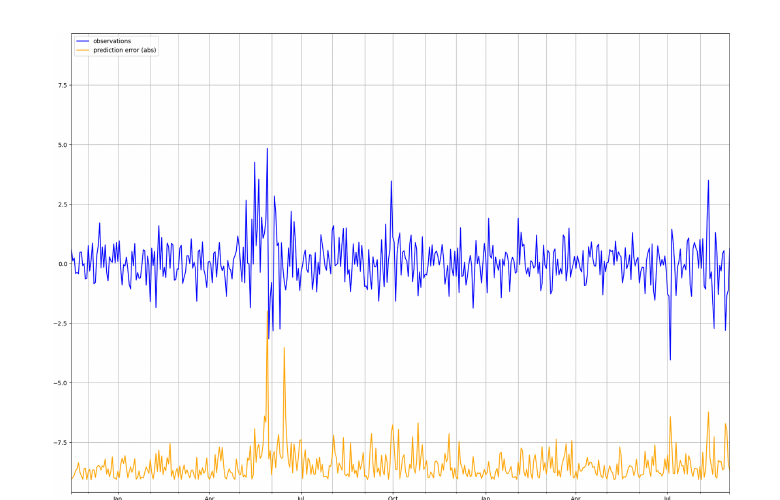
\includegraphics[width=0.85\linewidth]{gfx/m5l3_consoli_fig5.png}
\par\smallskip{\small \textbf{Hình 5.} Sai số dự báo tuyệt đối (MAFE) (màu cam) so với quan sát thực (màu xanh). (Nguồn: Consoli và cộng sự (2021), Hình 5)}
\end{figure}


Hiệu suất của mô hình giảm nhẹ từ cuối tháng 5 đến tháng 7/2018, tương ứng với giai đoạn bất ổn chính trị tại Ý. Thật vậy, ngày 29/5, chênh lệch lợi suất của Ý tăng mạnh, lên tới 250 điểm cơ bản. Nhà đầu tư đặc biệt lo ngại khả năng hình thành chính phủ chống đồng euro và thiếu niềm tin vào việc lập được một chính phủ ổn định. Từ tháng 6 đến tháng 11/2018, hàng loạt tranh luận về các cam kết chi tiêu thâm hụt và khả năng xung đột với các quy tắc tài khóa châu Âu tiếp tục khiến thị trường lo lắng. Chênh lệch lợi suất tăng mạnh vào tháng 10 và 11 với mức khoảng 300 điểm cơ bản. Điều này cũng thể hiện qua hiệu suất của mô hình, vốn giảm đôi chút trong giai đoạn căng thẳng này, nhưng nhìn chung mô hình vẫn xử lý khá tốt. Từ năm 2019, tình hình chính trị Ý bắt đầu cải thiện và chênh lệch lợi suất giảm dần, nhất là sau thỏa thuận với Brussels về thâm hụt ngân sách vào tháng 12/2018. Tuy nhiên, sau đó một số sự kiện đã tác động đến kinh tế Ý, như triển vọng tiêu cực của EU và cuộc bầu cử Nghị viện châu Âu, góp phần làm lãi suất tăng tạm thời. Trong giai đoạn này mô hình hoạt động khá tốt xét theo các tỷ lệ sai số tuyệt đối, cho thấy độ vững (robustness) tốt.

Hình 6 là biểu đồ phân tán giữa các điểm dự báo trung vị ngoài mẫu và các quan sát thực. Ở mức độ nào đó, các điểm trên biểu đồ bám khá sát đường chéo, cho thấy tương quan tốt giữa giá trị dự báo và quan sát thực, hàm ý chất lượng dự báo tốt. Điều này cũng được xác nhận bởi giá trị R-squared chấp nhận được là 0,23 trên các dự báo trung vị ngoài mẫu, đối với một bài toán dự báo nhiều thách thức như vậy. Giá trị R-squared này cho thấy mô hình LSTM giải thích được khá nhiều biến thiên của dữ liệu phản hồi quanh trung vị, gợi ý mức độ gần nhau nhất định giữa dữ liệu dự báo và quan sát thực.

\begin{figure}[H]
\centering
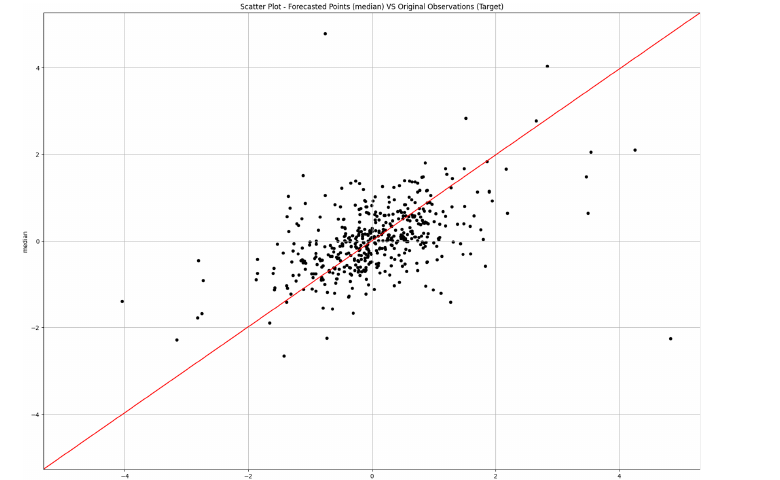
\includegraphics[width=0.85\linewidth]{gfx/m5l3_consoli_fig6.png}
\par\smallskip{\small \textbf{Hình 6.} Biểu đồ phân tán giữa các điểm dự báo trung vị ngoài mẫu và các quan sát thực. (Nguồn: Consoli và cộng sự (2021), Hình 6)}
\end{figure}


\section{6. Kết luận và triển vọng}

Bài báo trình bày công việc đang thực hiện về phương pháp xây dựng các chỉ báo kinh tế và tài chính thay thế, nắm bắt cảm xúc của nhà đầu tư và mức độ phổ biến của các chủ đề từ GDELT (Global Data on Events, Location, and Tone), một cơ sở dữ liệu nền tảng mở miễn phí chứa tin tức phát thanh, báo in và web toàn cầu theo thời gian thực. Dự án đang triển khai nhằm tạo ra các phương pháp dự báo cải tiến để phân tích thị trường trái phiếu chính phủ của các nước EU. Chúng tôi đã báo cáo một số kết quả sơ bộ khi áp dụng phương pháp này để dự báo thị trường trái phiếu chính phủ Ý. Trường hợp này cho thấy hiệu suất ban đầu tốt, gợi ý tính hợp lệ của cách tiếp cận. Nhờ sử dụng thông tin trích xuất từ truyền thông tin tức Ý trong GDELT kết hợp với mạng học sâu Long Short-Term Memory được huấn luyện và kiểm định phù hợp theo phương pháp cửa sổ trượt (rolling window), chúng tôi đã thu được kết quả dự báo khá tốt.

Đây là một trong những công trình đầu tiên nghiên cứu hành vi của chênh lệch lợi suất trái phiếu chính phủ và các quyết định danh mục đầu tư tài chính khi có mặt các nhân tố đường cong lợi suất cổ điển và thông tin trích xuất từ tin tức. Chúng tôi tin rằng các thước đo mới này có thể nắm bắt và dự báo các thay đổi trong động lực lãi suất, đặc biệt trong giai đoạn bất ổn. Nhìn chung, bài báo cho thấy cách dùng một cơ sở dữ liệu quy mô lớn như GDELT để xây dựng các chỉ báo tài chính nhằm nắm bắt ý định tương lai của các tác nhân trên thị trường trái phiếu chính phủ.

Chắc chắn cần nghiên cứu thêm theo các hướng đã nêu. Trước hết, chúng tôi sẽ cố gắng cải thiện hiệu suất của mô hình DeepAR đã triển khai bằng cách tinh chỉnh kiến trúc và tối ưu siêu tham số của mô hình LSTM. Ngoài ra, trong nghiên cứu hiện tại chúng tôi đang thử nghiệm các mô hình dự báo khác, từ phương pháp kinh tế truyền thống đến các phương pháp học máy mới, gồm Gradient Boosting Machines và các phương pháp dự báo bằng mạng nơ-ron. Trong phiên bản mở rộng sau này, chúng tôi sẽ so sánh và phân tích kỹ hiệu suất các phương pháp này để khai thác tốt hơn các tác động phi tuyến của các biến phụ thuộc. Khả năng diễn giải của các mô hình học máy, chẳng hạn bằng giá trị Shapley, sẽ là đối tượng nghiên cứu quan trọng trong tương lai nhằm đánh giá chính xác đóng góp của các biến đồng hành khác nhau vào dự báo của mô hình.

\textbf{Lời cảm ơn.} Các tác giả cảm ơn các đồng nghiệp tại Centre for Advanced Studies thuộc Joint Research Centre của Ủy ban châu Âu vì sự hướng dẫn và hỗ trợ hữu ích trong quá trình thực hiện nghiên cứu này.

\subsection{Tài liệu tham khảo}

\begin{enumerate}
\def\labelenumi{\arabic{enumi}.}
\item
  Agrawal, S., Azar, P., Lo, A.W., Singh, T.: Momentum, mean-reversion and social media: evidence from StockTwits and Twitter. J. Portfolio Manag. 44, 85--95
\end{enumerate}

\begin{enumerate}
\def\labelenumi{(\arabic{enumi})}
\setcounter{enumi}{2017}
\item
\end{enumerate}

\begin{enumerate}
\def\labelenumi{\arabic{enumi}.}
\setcounter{enumi}{1}
\item
  Alexandrov, A., et al.: GluonTS: probabilistic time series models in Python. CoRR, abs/1906.05264 (2019). http://arxiv.org/abs/1906.05264
\item
  Beber, A., Brandt, M.W., Kavajecz, K.A.: Flight-to-quality or flight-to-liquidity? Evidence from the Euro-area bond market. Rev. Financ. Stud. 22(3), 925--957
\end{enumerate}

\begin{enumerate}
\def\labelenumi{(\arabic{enumi})}
\setcounter{enumi}{2008}
\item
\end{enumerate}

\begin{enumerate}
\def\labelenumi{\arabic{enumi}.}
\setcounter{enumi}{3}
\item
  Benidis, K., et al.: Neural forecasting: introduction and literature overview. CoRR,
\end{enumerate}

abs/2004.10240 (2020). https://arxiv.org/abs/2004.10240

\begin{enumerate}
\def\labelenumi{\arabic{enumi}.}
\setcounter{enumi}{4}
\item
  Bernal, O., Gnabo, J.-Y., Guilmin, G.: Economic policy uncertainty and risk spillover in the Eurozone. J. Int. Money Finance 65(C), 24--45 (2016)
\item
  Borovykh, A., Bohte, S., Oosterlee, C.W.: Conditional time series forecasting with convolutional neural networks. Lecture Notes in Computer Science (including subseries Lecture Notes in Artificial Intelligence and Lecture Notes in Bioinformatics), vol. 10614, pp. 729--730 (2017)
\item
  Chang, Y.-C., Chang, K.-H., Wu, G.-J.: Application of eXtreme gradient boosting trees in the construction of credit risk assessment models for financial institutions. Appl. Soft Comput. J. 73, 914--920 (2018)
\item
  Deng, S., Wang, C., Wang, M., Sun, Z.: A gradient boosting decision tree approach for insider trading identification: an empirical model evaluation of china stock market. Appl. Soft Comput. J. 83 (2019)
\item
  Dridi, A., Atzeni, M., Reforgiato Recupero, D.: FineNews: fine-grained semantic sentiment analysis on financial microblogs and news. Int. J. Mach. Learn. Cybern., 1--9 (2018)
\item
  Favero, C., Pagano, M., von Thadden, E.-L.: How does liquidity affect government bond yields? J. Financ. Quant. Anal. 45(1), 107--134 (2010)
\item
  Garcia, A.J., Gimeno, R.: Flight-to-liquidity flows in the Euro area sovereign debt crisis. Technical report, Banco de Espana Working Papers (2014)
\item
  Gentzkow, M., Kelly, B., Taddy, M.: Text as data. J. Econ. Lit. (2019, to appear)
\item
  Gormley, C., Tong, Z.: Elasticsearch: The Definitive Guide. O' Reilly Media, Sebastopol (2015)
\item
  Hansen, S., McMahon, M.: Shocking language: understanding the macroeconomic effects of central bank communication. J. Int. Econ. 99, S114--S133 (2016)
\item
  Hochreiter, S., Schmidhuber, J.: Long short-term memory. Neural Comput. 9, 1735--1780 (1997)
\item
  Koenecke, A., Gajewar, A.: Curriculum learning in deep neural networks for financial forecasting. In: Bitetta, V., Bordino, I., Ferretti, A., Gullo, F., Pascolutti, S., Ponti, G. (eds.) MIDAS 2019. LNCS (LNAI), vol. 11985, pp. 16--31. Springer, Cham (2020). https://doi.org/10.1007/978-3-030-37720-5 2
\item
  Leetaru, K., Schrodt, P.A.: GDELT: global data on events, location and tone, 1979--2012. Technical report, KOF Working Papers (2013)
\item
  Liu, J., Wu, C., Li, Y.: Improving financial distress prediction using financial network-based information and GA-based gradient boosting method. Comput. Econ. 53(2), 851--872 (2019). https://doi.org/10.1007/s10614-017-9768-3
\item
  Loughran, T., McDonald, B.: When is a liability not a liability? Textual analysis, dictionaries and 10-ks. J. Finance 66(1), 35--65 (2011)
\item
  Manganelli, S., Wolswijk, G.: What drives spreads in the Euro area government bond markets? Econ. Policy 24(58), 191--240 (2009)
\item
  Mehdiyev, N., Enke, D., Fettke, P., Loos, P.: Evaluating forecasting methods by considering different accuracy measures. Procedia Comput. Sci. 95, 264--271 (2016)
\item
  Monfort, A., Renne, J.-P.: Decomposing Euro-area sovereign spreads: credit and liquidity risks. Rev. Finance 18(6), 2103--2151 (2013)
\item
  Nelson, C., Siegel, A.F.: Parsimonious modeling of yield curves. J. Bus. 60(4), 473--489 (1987)
\item
  Shah, N., Willick, D., Mago, V.: A framework for social media data analytics using Elasticsearch and Kibana. Wireless Networks (2018, in press)
\item
  Shapiro, A.H., Sudhof, M., Wilson, D.: Measuring news sentiment. Federal Reserve Bank of San Francisco Working Paper (2018)
\item
  Tetlock, P.C.: Giving content to investor sentiment: the role of media in the stock market. J. Finance 62(3), 1139--1168 (2007)
\item
  Thorsrud, L.A.: Nowcasting using news topics. big data versus big bank. Norges Bank Working Paper (2016)
\item
  Thorsrud, L.A.: Words are the new numbers: a newsy coincident index of the business cycle. J. Bus. Econ. Stat., 1--17 (2018)
\item
  Yang, X., He, J., Lin, H., Zhang, Y.: Boosting exponential gradient strategy for online portfolio selection: an aggregating experts' advice method. Comput. Econ. 55(1), 231--251 (2020). https://doi.org/10.1007/s10614-019-09890-2
\item
  Zhang, D., Hu, M., Ji, Q.: Financial markets under the global pandemic of COVID19. Finance Res. Lett., 101528 (2020)
\end{enumerate}

Giấy phép truy cập mở: Chương này được cấp phép theo Giấy phép Quốc tế Creative Commons Attribution 4.0 (http://creativecommons.org/licenses/by/4.0/), cho phép sử dụng, chia sẻ, phóng tác, phân phối và sao chép dưới mọi phương tiện hay định dạng, miễn là ghi nhận đúng tác giả gốc và nguồn, cung cấp liên kết tới giấy phép Creative Commons và nêu rõ các thay đổi (nếu có).

Hình ảnh hoặc tư liệu của bên thứ ba trong chương này thuộc giấy phép Creative Commons của chương, trừ khi có ghi chú khác trong phần ghi nguồn. Nếu tư liệu không thuộc giấy phép của chương và mục đích sử dụng của bạn không được quy định pháp luật cho phép hoặc vượt quá phạm vi cho phép, bạn cần xin phép trực tiếp chủ sở hữu bản quyền.
